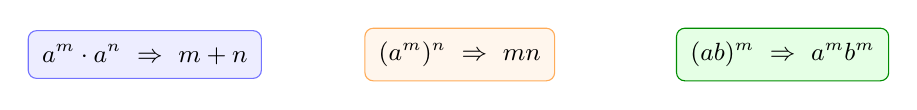
\begin{tikzpicture}[font=\small]
        \node[draw=blue!55,fill=blue!7,rounded corners=3pt,inner sep=5pt] at (0,0) {$a^m\cdot a^n\ \Rightarrow\ m+n$};
        \node[draw=orange!65,fill=orange!7,rounded corners=3pt,inner sep=5pt] at (4.0,0) {$(a^m)^n\ \Rightarrow\ mn$};
        \node[draw=green!55!black,fill=green!10,rounded corners=3pt,inner sep=5pt] at (8.1,0) {$(ab)^m\ \Rightarrow\ a^mb^m$};
    \end{tikzpicture}
